V priponskem drevesu nad besedo $T$ dolžine $n$ vsako vozlišče, pri čemer je $l$ listov in $v$ notranjih vozlišč, razen koren ima povezavo, ki kaže nanj. To lahko vidimo na zgornjem delu Slike \ref{fig:SuffuxArray}, na katerem je prikazano priponsko drevo za besedo \enquote{KOKOŠ$\$$}, da v vsako vozlišče kaže črna puščica. Vsako vozlišče razen korena ima tudi povezavo na svojega starša. Na sliki \ref{fig:SuffuxArray} teh povezan ni prikazani. Vsako notranje vozlišče v priponskem drevesu pa vsebuje tudi priponsko povezavo in le te so na Sliki \ref{fig:SuffuxArray} prikazane s sivo črtkano puščico. Torej priponsko drevo potrebuje $3v+2l-2$ povezav. Priponsko drevo ima $n$ listov in največ $n-1$ notranje vozlišče, torej priponsko drevo potrebuje med $2n+1$ in $5n -5$ povezav.

\begin{figure}[htb]
    \begin{subfigure}[t]{\linewidth}
        
        \includesvg[scale=.8]{Slike/KOKOŠMcCreightS1.svg}
        \centering
        \subcaption*{}
        \label{fig:bSADrevo}
    \end{subfigure}
    \begin{subfigure}[t]{1\linewidth}        
        \includesvg[scale=1.2]{Slike/KokosSA.svg}
        \centering
        \subcaption*{}
        \label{fig:bSAPolje}
    \end{subfigure}
    \caption{Primer priponskega drevesa in priponskega polja z dodatnim $LCP$ poljem nad besedo \enquote{KOKOŠ$\$$}.} 
    \label{fig:SuffuxArray}
\end{figure}

Vsaka povezava iz vozlišča $v_1$ v $v_2$, pri čemer je $\Stars{v_2}=v_1$, predstavlja ne prazen podniz besede $T$ in sicer podniz $\alpha$, ki je definiran kot $\Niz{v_2}=\Niz{v_1}\cdot\alpha$. To se lahko vidi na Sliki \ref{fig:SuffuxArray}, saj vsaka črna puščica ima zraven dopisan niz, ki ga predstavlja. Vsak podniz $\alpha$ je lahko predstavljen kot $T[s,e]$. Zato sta v vozlišču $v_2$ shranjena indeksa $s$ in $e$ z dvema celima številoma. Torej potrebuje priponsko drveo še prostora za shraniti $2(v+l-1)$ celih števil oziroma med $2n$ in $4n-2$ celih števil.

Vsak list v drevesu predstavlaj eno pripono, zato se v listih hrani še indeks začetka pripone v besedi. Z drugimi besedami, če je $i$ indeks pripone, ki jo predstavlja list $l$, potem velja, da je $\Niz{l}=T[i,n]$. To se lahko vidi tudi na Sliki \ref{fig:SuffuxArray}, kjer v vsakem listu je prikazan pripona, ki jo predstavlja. Zato predstaviti idekse začetkov pripon je porebinh še dodatnih $n$ celih šetvil. Če seštejemo vse skupaj priponsko drevo potrebuje največ $5n-5$ referenc na vozlišča in $5n-2$ celih števil ali $10n-7$ celih šetvil če se uporablja cela števila kot reference.

Pri tem pa se pojavi vprašanje, ali je mogoče indeksirati celotno besedo $T$ z zgolj $n$-timi celimi števili. Odgovor je da, saj vsak list v drevesu predstavlja eno pripono. To lahko storimo tako, da shrnimo indekse, ki so shranjeni v listih priponskega drevesa, v polju celih šetvil in sicer povnemo polje iz leve proti desni z indeki, ki jih dobimo ob premem sprehodu po drevesu. Pri tem pa se pojavi problem iskanja po takem polju, saj nam premi sprehod ne zagotavlja leksikografse urejenosti pripon. Brez škode za splošnost lahko predposvaimo, kot je bilo to storjeno na vseh slikah do zdej, da so povezave v priponskem drevesu leksikografsko urejene torej velja $\Niz{l_i}<\Niz{l_{i+1}}$. Torej imamo polje indeksov pripon, ki so leksigrafsko urejni, in to podatkovna struktura imenuje priponsko polje (angl. \textit{Suffix array} oziroma SA). Primer priponskega polja za besedo \enquote{KOKOŠ$\$$} je prikazan na spodnjem delu na Sliki \ref{fig:SuffuxArray}. Poleg priponskega polja označenega $SA$ je prikazna na sliki tudi $LCP$ polje.


%Priponsko polje je alternativni indeks besedila. Priponsko polje se uporablja namesto priponskega drevesa, ko se potrebuje prostorsko bolj učinkovito podatkovno strukturo in se lahko žrtvuje čas iskanja vzorcev v besedilu saj priponsko polje zasede približno 8-krat manj prostora na delovnem pomnilniku kot priponsko drevo \cite{Manber1990}. Priponsko polje si lahko predstavljamo kot polje listov priponskega drevesa, brez podatkov o notranjih vozliščih drevesa. To podobnost lahko vidimo tudi na Sliki \ref{fig:SuffuxArray}, na kateri je prikazano priponsko drevo in priponsko polje za besedo \enquote{KOKOŠ$\$$}.

V nadaljevanju poglavja bodo predstavljena implementacija poized nad vhodno besedo s pomočjo priponskega polja ter pospešitev iskanja z dodatno podatkovno strukturo imenovano LCP polje. Za tem bo predstavljena posplošitev LCP polja, ki omogoča simuliranje priponskega drevesa. Nato pa bo predstavlje še način gradnje priponskega polja.

%\begin{figure}[htb]
%    \begin{center}
%        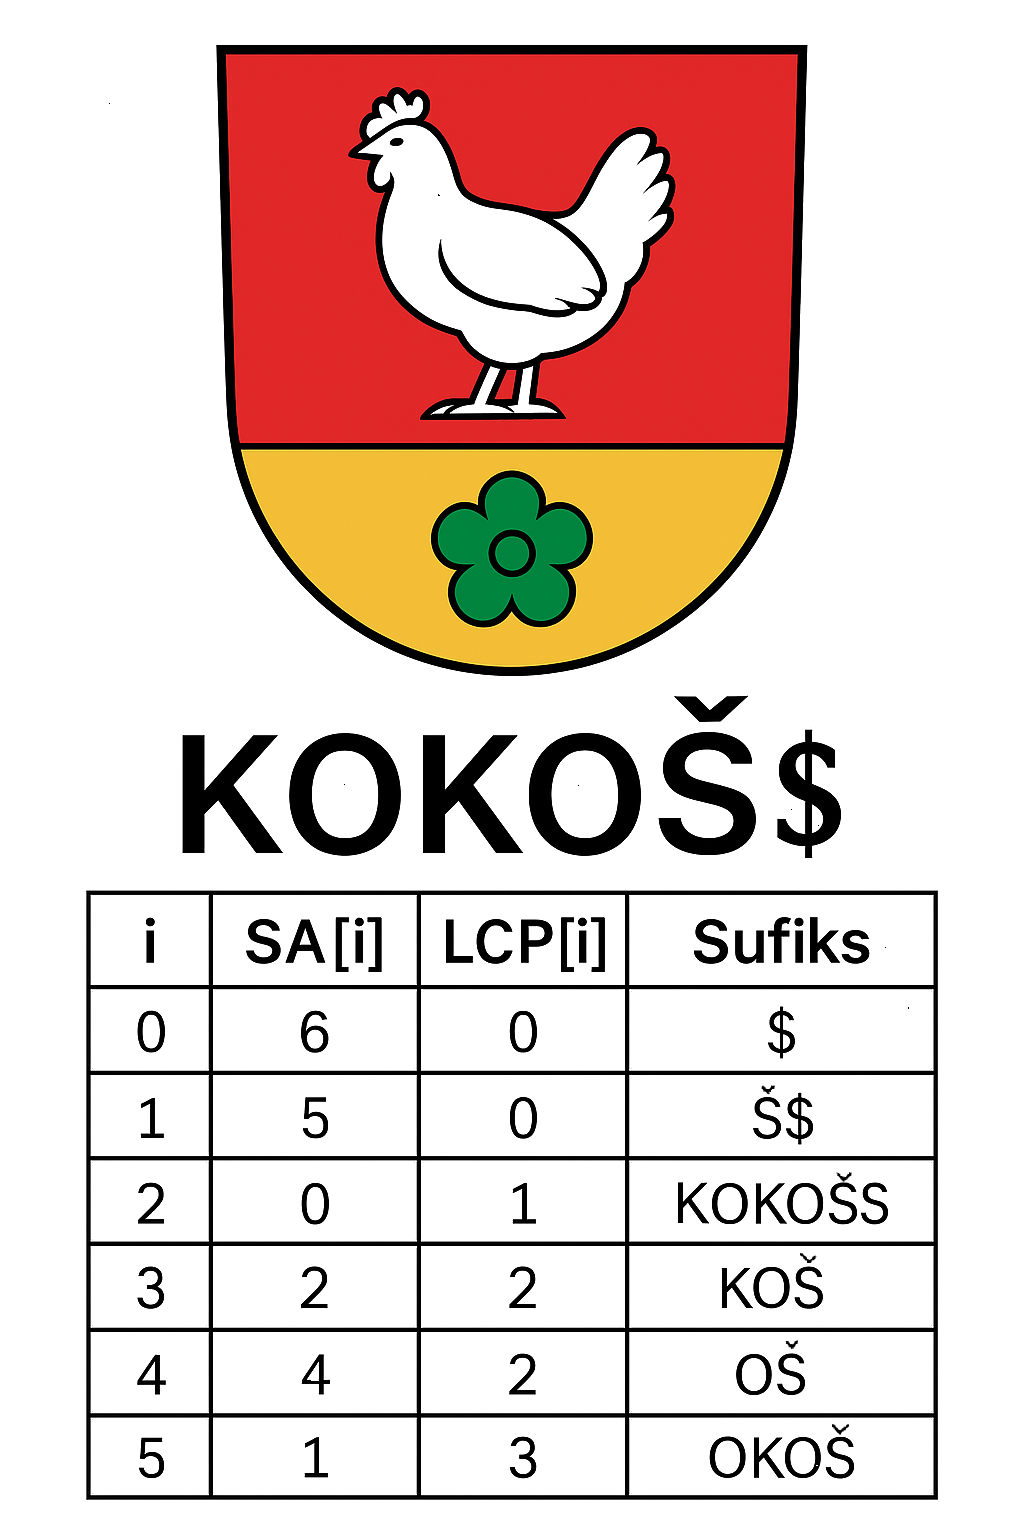
\includegraphics[width=.5\textwidth]{Slike/ChatGPTSA.png}
%        \caption{Primer priponskega polja nad besedo \enquote{KOKOŠ$\$$} kot si jo predstavlja ChatGPT.} 
%        \label{fig:ChatGPT}
%    \end{center}
%\end{figure}



%\section{NAJDALJŠA SKUPNA PREDPONA}\label{sec:LCP}
%\import{.}{PriponskoPolje/LCP}

\section{POIZVEDBE}\label{sec:SAPoizvedbe}
\import{.}{PriponskoPolje/Poizvedba}


\section{IZGRADNJA}\label{sec:SAIzgradnja}
\import{.}{PriponskoPolje/Izgradnja}




\section{SIMULACIJA PRIPONSKEGA DREVESA}\label{sec:STsimulacija}
\import{.}{PriponskoPolje/SimulacijaDrevesa}